\documentclass[t]{beamer}

% Load general definitions
\input{../defs/preamble.tex}
\usecolortheme{crane}

% Specific definitions
\title[]{Experiment Design for Computer Sciences}
\subtitle[]{00 - Course Intro -- Tsukuba Specific Notes}
\author[]{Claus Aranha\\{\footnotesize \url{http://conclave.cs.tsukuba.ac.jp/}}}
\institute{Computer Science Department}
\date{\scriptsize Tsukuba, 2016}

\begin{document}

% cover page
\setbeamertemplate{footline}{}
\begin{frame}
\begin{flushright}
%\includegraphics[width=.25\textwidth]{../figs/principal_completa3_ufmg}
\end{flushright}
  \titlepage
  \begin{tikzpicture}[remember picture,overlay]
  \node[anchor=south east,xshift=-5pt,yshift=122pt] at (current page.south east) {\tiny Version 2.11.T};
  \node[anchor=south west,yshift=0pt] at (current page.south west) {\includegraphics[width=.15\textwidth]{../figs/by-nc-sa.png}};
  \end{tikzpicture}  
\end{frame}

% Main slides
\begin{ftst}
{Lecturer Introduction}
{Who am I?}
\begin{columns}[T]
  \column{0.4\textwidth}
  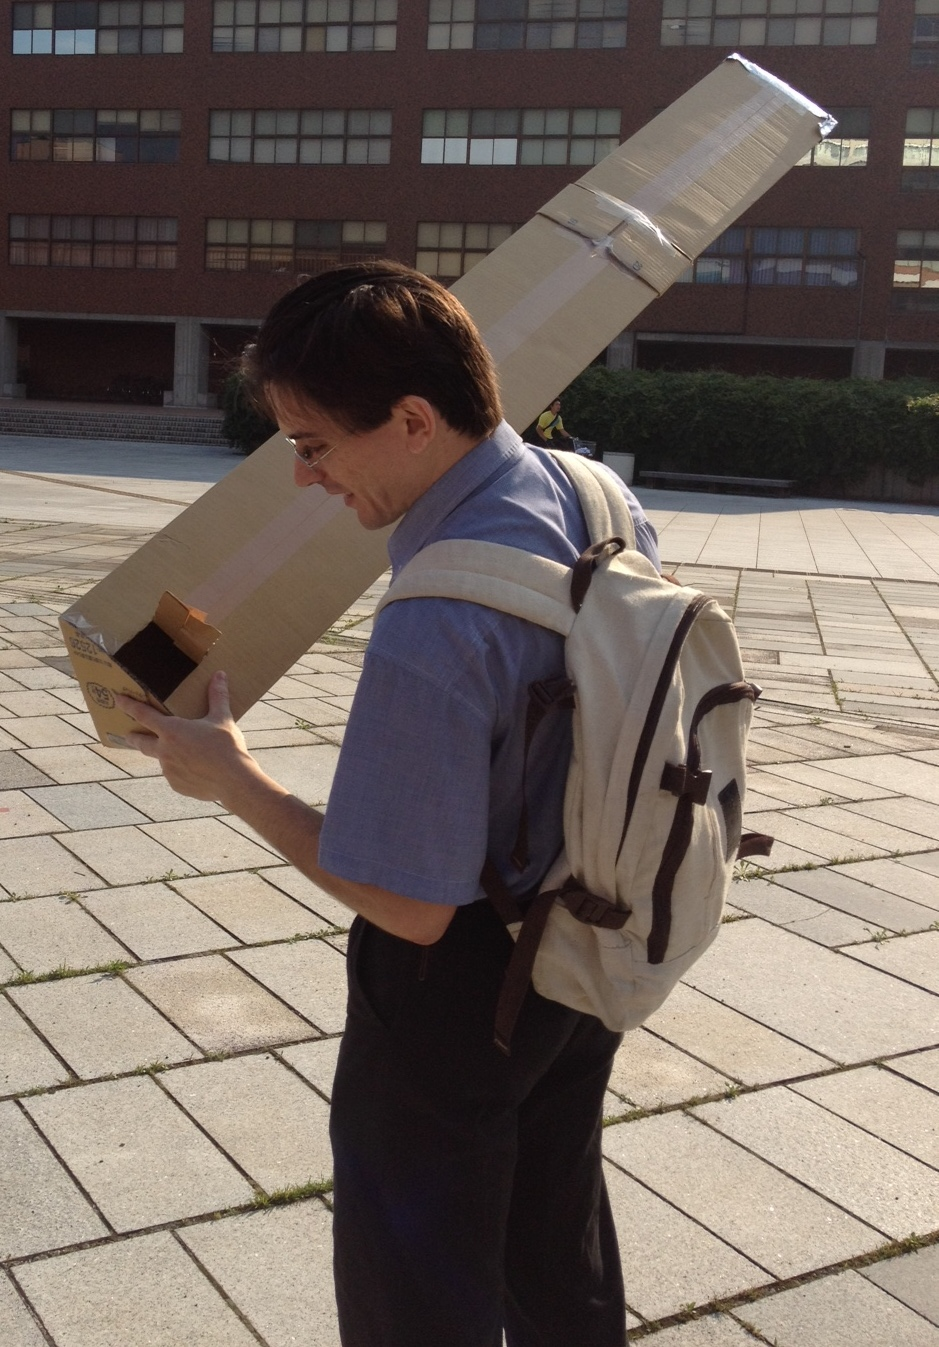
\includegraphics[width=1\textwidth]{../figs/pinhole}
  \column{0.6\textwidth}
  \bitems \structure{Name:} Claus Aranha;
  \item \structure{Country:} Brazil;
  \spitem \structure{Research:} Artificial Intelligence, Genetic
  Algorithms, Deep Learning;
  \item \structure{Language:} Python, R;
  \item \structure{Hobbies:} Game Programming, Geocaching, Twitter
    Bots;

  \spitem \structure{twitter:} \href{http://www.twitter.com/caranha}{@caranha}
  \item \url{http://conclave.cs.tsukuba.ac.jp}
  \eitem
\end{columns}
\end{ftst}

\begin{ftst}
{Motivation for this course}{Why am I doing this?}  

% TODO: Add a silly figure here
% TODO: List more concrete examples in notes 
% (and hope I can remember everything!)

I want to fix a problem:
\vone
\begin{itemize}
  \item Low quality of student papers;
  \item Low awareness of bad references;
  \item Low awareness of bad practices;
  \item Good will, sloppy execution
  \item End result: A lot of wasted work!
\end{itemize}

\vfill

{\bf Very} recommended read: \url{http://www.statisticsdonewrong.com/}
\end{ftst}

\begin{ftst}
{Materials}{Github Repository Structure}
{\small \url{https://github.com/caranha/Design-and-Analysis-of-Experiments}}
\begin{itemize}
  \item \emph{XX-Chapter} -- Text for one class
    \begin{itemize}
    \item \emph{ChapterXX.pdf} -- Main notes
    \item \emph{ChapterXX-Tsukuba.pdf} -- Special notes for our course
    \end{itemize}
  \item \emph{data files} -- Data for exercises/examples
  \item \emph{DemoXX} -- Software demos for CLT and CI
  \item \emph{Forms/Grading} -- Not used for this course (yet)
  \item \emph{Refence Material} -- Some useful PDFs/Links
  \item \emph{TSUKUBA/figs/defs} -- Maintenance files    
\end{itemize}

\begin{block}{Note: Old Repository}
  {\small \url{https://github.com/caranha/ExperimentDesignLectureNotes}}\\
  \vhalf
  Will not be used this semester, but you migth check it out for extra info.
\end{block}
\end{ftst}

\begin{ftst}
{Materials}{MANABA}

For this class, we will make intensive use of the MANABA e-learning
system: Report Submission, Class Announcements, Discussion.
\vone
\bitems Manaba Webpage: \url{https://manaba.tsukuba.ac.jp/ct/course_578828}
\item Manaba Enrollment Code: 5718071 
\eitem
\vone 

There is already a survey in the system - Please take the time to
answer it during the weekend.
\end{ftst}

\begin{ftst}
{Calendar}{Planned class dates -- May still change}
\bitems 04/15 Lecture -- (00,01,02)
\item 04/22 Lecture -- (03)
\item 05/06 Lecture -- TBD
\item 05/13 Lecture -- TBD
\item 05/20 Lecture -- TBD
\item 06/03 Lecture -- TBD
\item 06/10 Lecture -- TBD
\item 06/17 Lecture -- TBD
\item 06/24 Lecture -- TBD
\spitem 07/01 *Substitute Lecture*
\item 07/08 Final Presentation
\eitem
\end{ftst}

\begin{ftst}
{Calendar}{Class Structure}
- Class Structure
  - 3 hours is TOO much time
  - A- question about readings, projects, previous class
  - B- lecture itself
  - C- Questions, repetitions
  - D- Work on data, examples, extra information
  - E- We will frequently end the class early.
\end{ftst}

\begin{ftst}
{English Program}{Please register!}

The ``Computer Science English Program'' promotes the establishment of
lecturer in English in our department. To evaluate the demand for these 
courses, we ask you to please enroll in the CSE.
\vone
\begin{block}{How to Enroll in CSE}
Send an e-mail to \alert{s-g30@cs.tsukuba.ac.jp} with:\\
\vone
\bitems Subject: Enrollment in CSE Program
\item Contents: Name, Student Number
\eitem
\end{block}
\vone
\begin{center}
  Deadline: May 15th (Friday)
\end{center}
\end{ftst}

\begin{ftst}
{English Program}{Academic Writting/Speaking classes}
\begin{block}{}
Attention: Report grading will include ``clear writing''
\end{block}

\vone

If you are unsure of your writing ability in English, 
consider enrolling in some of the following courses.

\vone

\bitems Introductory Technical Writing: 02CA101
\item Advance Technical Writing: 02CA103
\item Science Communication I: 02CA105
\item Science Communication II: 02CA107
\eitem

\vone

For more information about these courses, contact professor
Neil Millar (millar@cs.tsukuba.ac.jp).
\end{ftst}

\end{document}
